\documentclass[11pt,a4paper]{article}
\usepackage[a4paper,hmargin=1in,vmargin=1in]{geometry}
\usepackage{pgfplots}
\pgfplotsset{compat=1.17}

\usepackage[czech]{babel}
\usepackage[utf8]{inputenc}
\usepackage[T1]{fontenc}

\usepackage{stddoc}
\usepackage{lipsum}
\usepackage{subcaption}

\newcommand{\plus}{{\texttt{+}}}
\renewcommand{\Re}{\operatorname{Re}}
\renewcommand{\Im}{\operatorname{Im}}
\newcommand{\fourier}[3]{\mathcal{F}_{#1}\!\left[#2\right]\!\left(#3\right)}
\newcommand{\ifourier}[3]{\mathcal{F}^{-1}_{#1}\!\left[#2\right]\!\left(#3\right)}


\begin{document}

\pagenumbering{arabic}

% Header
\begin{center}
    {\LARGE\textbf{Laboratorní úloha č. 3}}\\[3mm]
    \begin{minipage}{0.4\textwidth}
        \begin{flushleft}
            \textsc{\today}
        \end{flushleft}
    \end{minipage}
    ~
    \begin{minipage}{0.4\textwidth}
        \begin{flushright}
            \textsc{Martin Šimák}
        \end{flushright}
    \end{minipage}
    \noindent\rule{14.5cm}{0.4pt}
\end{center}

\paragraph*{Téma} Měření velkosignálových vlastností mikrovlnných zesilovačů

Cílem této úlohy bylo seznámit se s měřením velkosignálových vlastností mikrovlnných zesilovačů. To zahrnuje pozorování a popis nelineárního chování jako je saturace, bod decibelové komprese a přítomnost intermodulačních produktů při směšování signálů.


\subsection*{Úkoly měření}
\begin{enumerate}%[label=\arabic*.]
    \item Bod decibelové komprese $P_{1\mathrm{dB}}$ zesilovačů.
    \item Bod zahrazení IP3 pro složky $2a+b$ zeilovačů.
\end{enumerate}


\subsection*{Použité přístroje a komponenty}
\begin{itemize}
    \item Spektrální analyzátor R\&S FSP30 (9~kHz až 30~GHz)%
        \footnote{Zápis jednotek a rozsahů hodnot pomocí slova až (angl. \emph{to}) namísto pomlčky (--) jsem zvolil po vzoru doporučení pro zápis jednotek SI, \url{https://physics.nist.gov/cuu/pdf/sp811.pdf}, sekce 7.7.}
    \item Generátor R\&S SMIQ 03B (300~kHz až 3,3~GHz)
    \item Generátor Agilent E8257D (250~kHz až 50~GHz)
    \item Elektronicky řiditelné atenuátory HP 84904L a 84906L (0~Hz až 40~GHz)
    \item Koaxiální dolní propust Mini-Circuits RPS-2-30\plus~(0~Hz až 1050~MHz)
    \item Dělič výkonu/slučovač Mini-Circuits ZX10-2-20-S\plus~(200~MHz až 2000~MHz)
    \item Propojovací SMA kabel Mini-Circuits CBL-2FT-SMSM\plus
    \item Dva propojovací kabely Pasternack PE300-36
\end{itemize}


\subsection*{Měřené zesilovače}
\begin{itemize}
    \item Mini-Circuits ERA-3SM\plus
    \item Nízkošumový zesilovač s tranzistorem NXP BFU-760F
\end{itemize}

\subsection*{Postup měření}
Zapojení úlohy vhodné pro tato měření je patrné z obrázku \ref{fig:connection-scheme}. Spektrální analyzátor je s oběma generátory spojen pomocí BNC kabelů s referenčním signálem o frekvenci 10~MHz, aby generátory generovaly koherentní signál a analyzátor detekoval signály s přesnou frekvencní. Zdrojem reference je v tomto zapojení spektrální analyzátor R\&S a generátory jsou nastaveny, aby tento externí signál braly jako referenční místo svého interního zdroje.

\begin{figure}[!ht]
\begin{center}
    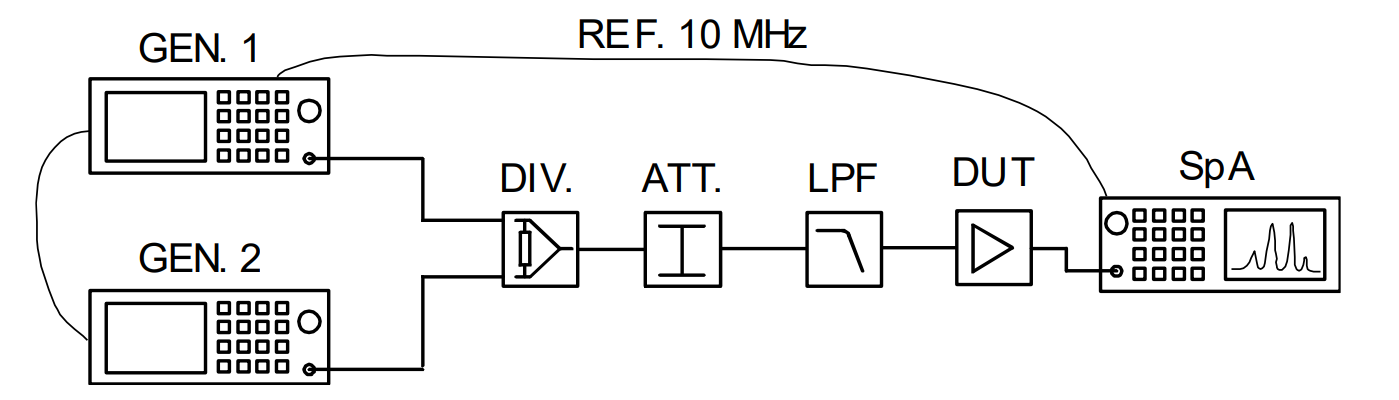
\includegraphics[width=0.8\textwidth]{src/connection-scheme.png}
\end{center}
\caption{Schéma zapojení úlohy}
\label{fig:connection-scheme}
\end{figure}

Pro měření intermodulačních produktů zesilovačů je potřeba zajistit co nejčistší výstupní signál generátorů. Na výstup externích atenuátorů je proto připojena koaxiální dolní propust VLFX-1050\plus. Kaskáda použitch kabelů, slučovače, atenuátorů (s útlumem nastaveným na 0~dB) a filtru je zhruba 6~dB, což kompenzujeme dostavením výkonů obou generátorů.

Jelikož měření decibelové komprese a intermodulačních produktů zesilovačů probíhá v režimu blízko saturace měřeního zesilovače, vyžaduje úloha měření relativně velkých výkonů. Lze předpokládat, že maximální měřený výkon bude 10~dBm. Analyzátor je proto potřeba nastavit tak, aby takový výkon nepřebudil vstupní obvody, zejména první směšovač. V opačném případě by vstupní obvod analyzátoru sám generoval intermodulační produkty nerozeznatelné od těch, které generuje měřený zesilovač. Takové nastavení lze dosáhnout zapnutím obou generátorů zároveň, což způsobí výskyt intermodulačních produktů 3. řádu na obrazovce spektrálního anayzátoru. Jelikož všechny externí komponenty jsou obvody lineární a intermodulační produkty na nich tedy nevznikají, utlumíme je pomocí vstupního atenuátoru spektrálního analyzátoru. V tuto chvíli máme jistotu, že i při měření signálů o výkonu 10~dBm bude přijímač spektrálního analyzátoru provozován v lineárním řežimu, a tak budeme decibelovou kompresi i intermodulační produkty zesilovačů měřit přesně.

\paragraph*{Bod decibelové komprese zesilovačů}
Nejprve je třeba nastavit na obou generátorech výkony tak, aby spektrální analyzátor měřil výkony 0~dBm. Útlum atenutárorů zatím ponecháváme na 0~dB. Jen tak si můžeme být jisti, že na vstup měřených zesilovačů bude přiváděn výkon číselně roven $-L_{\mathrm{att}}$, kde $L_{\mathrm{att}}$ je nastavený útlum externích atenuátorů.

\begin{table}[!ht]
\begin{center}
\begin{tabular}{| l || c | c | c | c | c | c | c | c | c | c | c |}
    \hline
    $L_{\mathrm{att}}$ [dB] & 30 & 25 & 20 & 15 & 11 & 9 & 8 & 7 & 6 & 5 \\
    \hline
    $P_{\mathrm{out}}$ [dBm] & -10,5 & -5,1 & -0,2 & 4,8 & 8,6 & 10,4 & 11,1 & 11,7 & 12,3 & 12,7 \\
    \hline\hline
    $G$ [dB] & 19,5 & 19,9 & 19,8 & 19,8 & 19,6 & 19,4 & 19,1 & 18,7 & 18,3 & 17,7 \\
    \hline
\end{tabular}
\caption{Hodnoty pro určení $P_{1\mathrm{dB}}$ zesilovače ERA-3SM\plus}
\label{table:ERA3SM-compression}
\end{center}
\end{table}

\begin{table}[!ht]
\begin{center}
\begin{tabular}{| l || c | c | c | c | c | c | c | c | c | c | c |}
    \hline
    $L_{\mathrm{att}}$ [dB] & 30 & 25 & 20 & 15 & 13 & 12 & 11 & 10 & 9 & 8 \\
    \hline
    $P_{\mathrm{out}}$ [dBm] & -9,9 & -4,5 & 0,4 & 5,3 & 7 & 7,8 & 8,8 & 9,5 & 10,1 & 10,5 \\
    \hline\hline
    $G$ [dB] & 20,1 & 20,5 & 20,4 & 20,3 & 20 & 19,8 & 19,8 & 19,5 & 19,1 & 18,5 \\
    \hline
\end{tabular}
\caption{Hodnoty pro určení $P_{1\mathrm{dB}}$ LNA s tranzistorem BFU-760F}
\label{table:BFU760F-compression}
\end{center}
\end{table}

Necháme zapnutý pouze generátor s frekvencí 1~GHz a za počátečního útlumu externích atenutárorů 30~dB připojíme jeden z měřených zesilovačů. Napájecí napětí zesilovače je 12~V a proudová pojistka 100~mA. Pomocí markeru na spektrálním analyzátoru s dostatečně širokým nastaveným rozsahem frekvenční (0,5~GHz až 3,5~GHz) čteme hodnoty výkonu výstupního signálu zesilovače na frekvenci 1~GHz a jsou zřetelné i vyšší harmonické složky. Další měření spočívá v postupném snižování útlumu externích atenutárorů tak, abychom proměřili závislst výstupního výkonu zesilovače $P_{\mathrm{out}}$ na vstupním výkonu $P_{\mathrm{in}}$ až k saturaci zesilovače. Naměřené hodnoty jsou zaznamenané v tabulkách~\ref{table:ERA3SM-compression}~a~\ref{table:BFU760F-compression} pro jednotlivé zesilovače. Grafické znázornění nejprve lineárního chování dynamického rozsahu zesilovačů i následný bod decibelové komprese $P_{1\mathrm{dB}}$ a saturace jsou znázorněny na obrázcích~\ref{fig:ERA3SM-compression}~a~\ref{fig:BFU760F-compression}.

\begin{figure}[!ht]
\begin{subfigure}{0.5\textwidth}
    \centering
    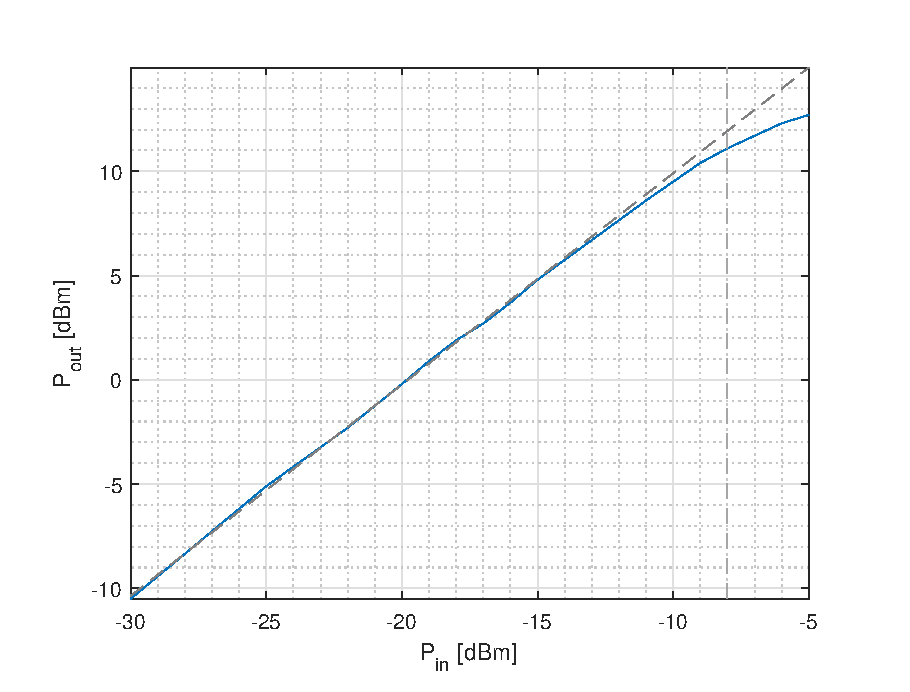
\includegraphics[width=\textwidth]{src/ERA3SM-compression.eps}
    \caption{ERA-3SM\plus}
    \label{fig:ERA3SM-compression}
\end{subfigure}%
\begin{subfigure}{0.5\textwidth}
    \centering
    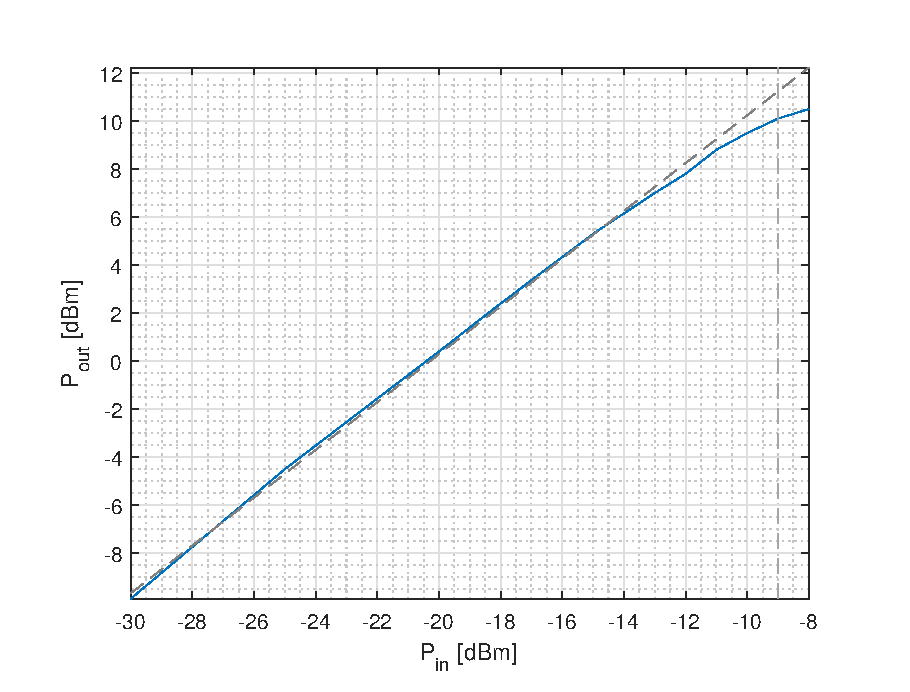
\includegraphics[width=\textwidth]{src/BFU760F-compression.eps}
    \caption{LNA s BFU-760F}
    \label{fig:BFU760F-compression}
\end{subfigure}
\caption{Grafické zpracování dat pro ilustraci decibelové komprese}
\end{figure}

Vztaženo k výstupu zesilovačů je hodnota $P_{1\mathrm{dB}} = 11,1~\mathrm{dBm}$ pro zesilovač ERA-3SM\plus~a pro nízkošumový zesilovač s tranzistorem BFU-760F je $P_{1\mathrm{dB}} = 10,1~\mathrm{dBm}$.

\paragraph*{Bod zahrazení intermodulačními produkty třetího řádu}
Schéma zapojení a nastavení vstupních obvodů spektrálního analyzátoru je ponecháno z předchozího úkolu.

Po zapnutí výstupů z obou generátorů a počátečním nastavením útlumu externích atenuátorů na 25~dB%
    \footnote{Na doporučených 30~dB nebyly intermodulační produkty ještě dostatečně čitelné z šumového pozadí.}
lze na obrazovce spektrálního analyzátoru číst hodnoty výkonů základní harmonické $P_a$ a intermodulačních produktů $P_{2a\pm b}$. Z toho lze dále spočítat výkonový odstup intermodulačních produktů od základní harmonické $O_{2a\pm b}$. Změřené a výpočtené hodnoty měření jsou zaznamenané v tabulkách~\ref{table:ERA3SM-intercept}~a~\ref{table:BFU760F-intercept} pro jednotlivé zesilovače. Vývoj hodnot výkonů a následný bod zahrazení IP3 pro složky $2a \pm b$ jsou znázorněny na obrázcích~\ref{fig:ERA3SM-intercept}~a~\ref{fig:BFU760F-intercept}.

\begin{table}[!ht]
\begin{center}
\begin{tabular}{| l || c | c | c | c | c | c | c | c | c | c | c |}
    \hline
    $L_{\mathrm{att}}$ [dB] & 23 & 20 & 17 & 15 & 14 & 11 & 8 & 7 & 5 & 2 \\
    \hline
    $P_a$ [dBm] & -3,2 & -0,2 & 2,7 & 4.6 & 5,5 & 7,6 & 8,9 & 9.2 & 9,6 & 10,1 \\
    \hline
    $P_{2a \pm b}$ [dBm] & -60 & -50,6 & -40,7 & -33,4 & -29,7 & -17,8 & -10,6 & -9,4 & -7,5 & -7,6 \\
    \hline\hline
    $O_{2a \pm b}$ [dBm] & 56,8 & 50,4 & 43,4 & 38 & 35,2 & 25,4 & 19,5 & 18,6 & 17,1 & 17,7 \\
    \hline
\end{tabular}
\caption{Hodnoty pro určení IP3 zesilovače ERA-3SM\plus}
\label{table:ERA3SM-intercept}
\end{center}
\end{table}

\begin{table}[!ht]
\begin{center}
\begin{tabular}{| l || c | c | c | c | c | c | c | c | c | c | c |}
    \hline
    $L_{\mathrm{att}}$ [dB] & 25 & 22 & 19 & 16 & 13 & 11 & 10 & 9 & 7 & 4 \\
    \hline
    $P_a$ [dBm] & -4,5 & -1,75 & 1,3 & 3,8 & 6 & 7 & 7,2 & 7,3 & 7,3 & 7,1 \\
    \hline
    $P_{2a \pm b}$ [dBm] & -57 & -48 & -34,7 & -23,6 & -16,6 & -15,6 & -16,2 & -16,1 & -11,7 & -5,7 \\
    \hline\hline
    $O_{2a \pm b}$ [dBm] & 52,5 & 46,25 & 36 & 27,4 & 22,6 & 23,1 & 22,8 & 23,5 & 19 & 12,8 \\
    \hline
\end{tabular}
\caption{Hodnoty pro určení IP3 LNA s tranzistorem BFU-760F}
\label{table:BFU760F-intercept}
\end{center}
\end{table}

\begin{figure}[!ht]
    \centering
\begin{subfigure}{0.45\textwidth}
    \centering
    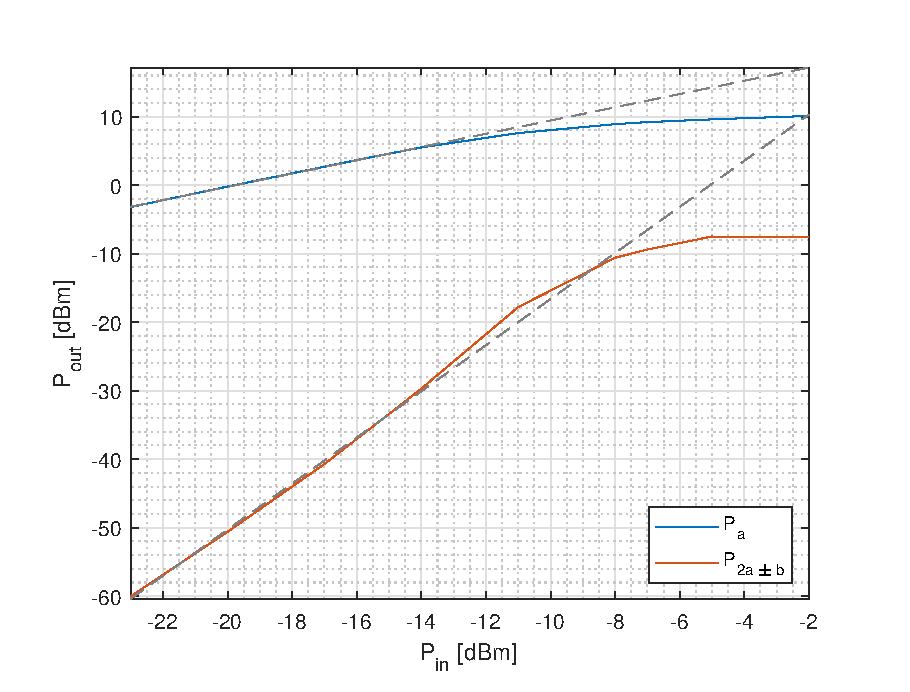
\includegraphics[width=\textwidth]{src/ERA3SM-intercept.eps}
    \caption{ERA-3SM\plus}
    \label{fig:ERA3SM-intercept}
\end{subfigure}
\begin{subfigure}{0.45\textwidth}
    \centering
    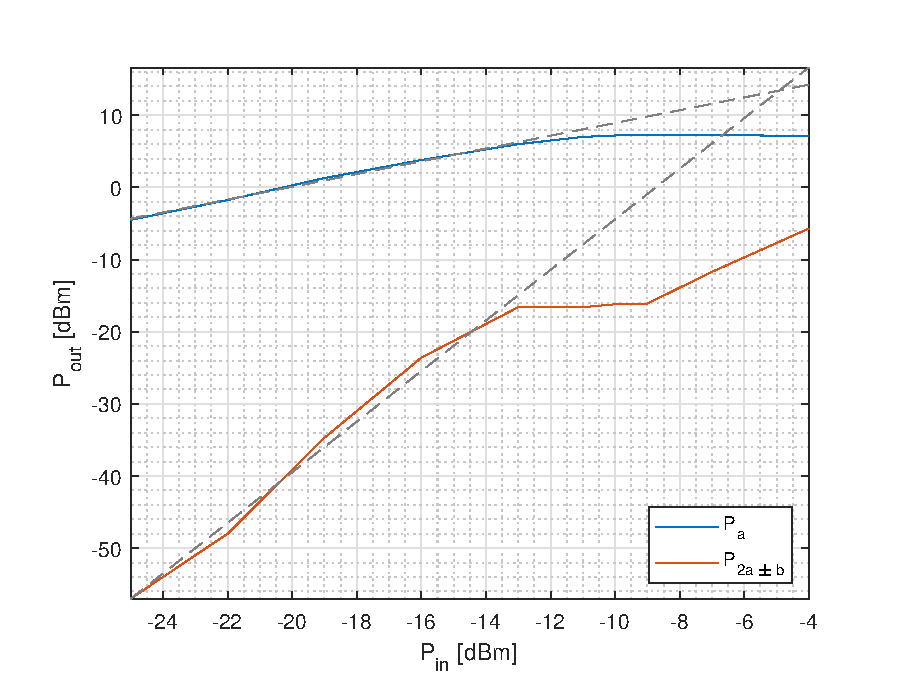
\includegraphics[width=\textwidth]{src/BFU760F-intercept.eps}
    \caption{LNA s BFU-760F}
    \label{fig:BFU760F-intercept}
\end{subfigure}
\caption{Grafické zpracování dat pro ilustraci zahrazení IM3}
\end{figure}

Vztaženo k výstupu zesilovačů je hodnota $P_{\mathrm{IP3}} = 20~\mathrm{dBm}$ pro zesilovač ERA-3SM\plus~a pro nízkošumový zesilovač s tranzistorem BFU-760F je $P_{\mathrm{IP3}} = 13,4~\mathrm{dBm}$.

\subsection*{Závěr}
V rámci úlohy jsme se seznámili se základy měření velkosignálových vlastností mikrovlnných zesilovačů jako jsou bod decibelové komprese a bod zahrazení IP3. Během úlohy jsme nenarazili na žádné výrazné překážky, a tak se nám podařilo si ověřit teoretické znalosti dynamického rozsahu mikrovlnných systémů.

Měřením byly zjištěny hodnoty $P_{1\mathrm{dB}} = 11,1~\mathrm{dBm}$, $P_{\mathrm{IP3}} = 20~\mathrm{dBm}$ pro zesilovač ERA-3SM\plus~a pro LNA s tranzistorem BFU-760F $P_{1\mathrm{dB}} = 10,1~\mathrm{dBm}$, $P_{\mathrm{IP3}} = 13,4~\mathrm{dBm}$.

Dlužno podotknout, že v případě bodu decibelové komprese se jedná přímo o reálné hodnoty výstupního výkonu zesilovačů, zatímco bod IP3 je samozřejmě pouze teoretickou hodnotou, která byla získána jako průsečík prodloužení lineárních tendencí závislosti výstupního výkonu žádoucího signálu a intermodulačních produktů 3. řádu před jejich deklinací.

\end{document}
